\section{Minimax}
\begin{figure}
    \centering
    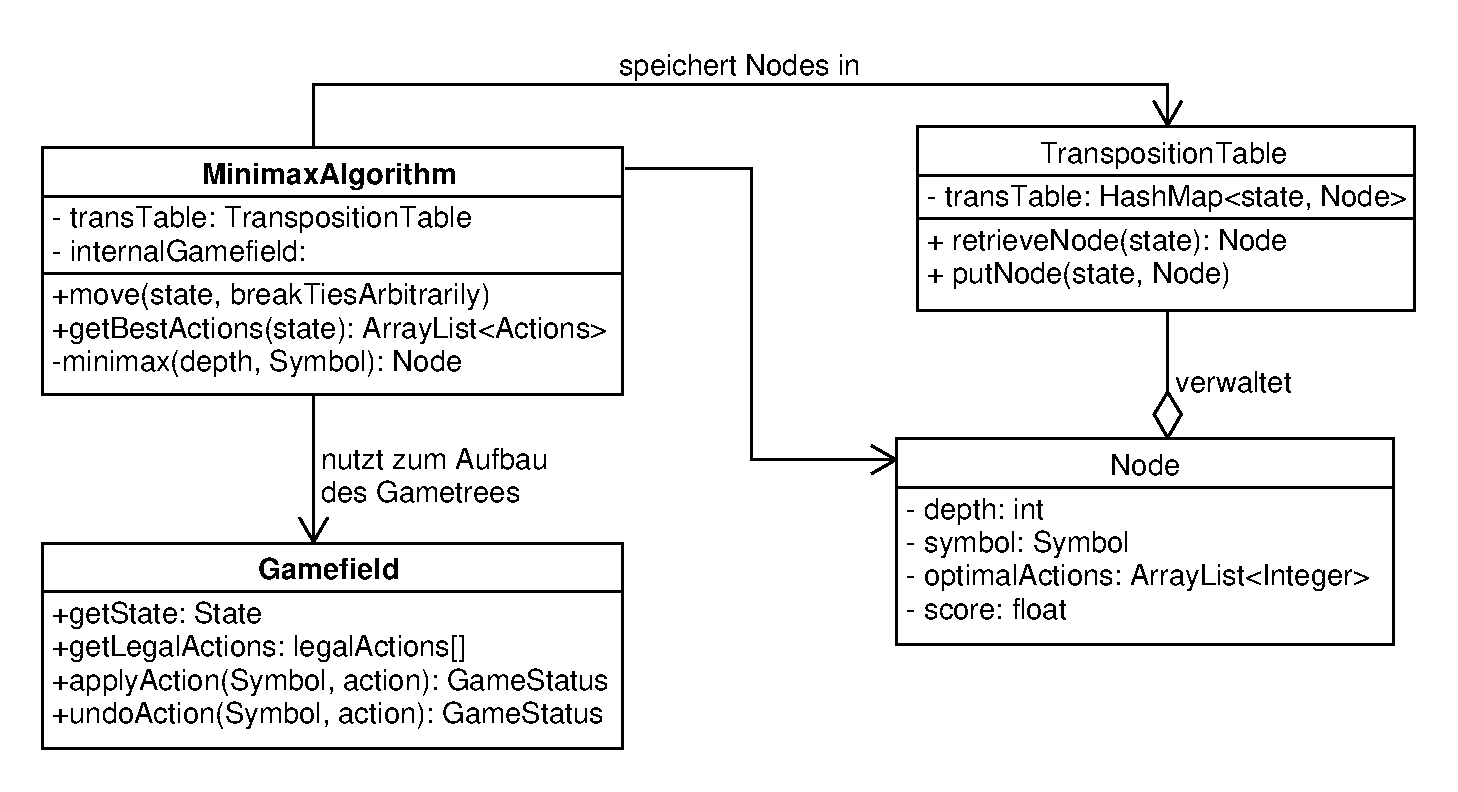
\includegraphics[width=\textwidth]{04_Artefakte/01_Abbildungen/uml/uml_minimax.pdf}
    \caption{MinimaxAlgorithm und verbundene Klassen}
    \label{fig:uml_minimax}
\end{figure}

\cref{fig:uml_minimax} zeigt die wichtigsten Bestandteile der MinimaxAlgorithm-Klasse sowie deren Interaktion mit anderen Klassen.
MinimaxAlgorithm implementiert den Minimax-Algorithmus aus \cref{sec:minimax} und dient der Evaluation der Agenten. 
Einerseits wird während des Trainings geprüft, ob die vom Agenten gewählten Aktionen optimal sind. 
Andererseits ist Minimax ein Gegner im Rahmen der Evaluationsspiele, um die Spielstärke der Agenten zu messen. 

Die Klasse bietet dafür zwei Methoden. 
Für die Bewertung der Aktionen des Agenten gibt es die getBestActions-Methode. 
Diese gibt alle gleich optimalen Aktionen zu einem Zustand zurück, sodass geprüft werden kann, ob die vom Agenten gewählte Aktion ein Element dieser Liste und somit optimal ist. 
Die move-Methode gibt für einen Zustand eine der optimalen Aktionen zurück, sodass Minimax als Gegner genutzt werden kann. 
Dabei kann als zweiter Parameter übergeben werden, ob bei mehreren gleich optimalen Aktionen die Aktion mit dem niedrigsten Index oder eine zufällige ausgewählt werden soll. 
Da in den Evaluationsspielen möglichst viele unterschiedliche Zustände betrachtet werden sollen, wird die Option für nichtdeterministisches Spiel genutzt.

Der Spielbaum wird konstruiert durch die minimax-Methode, die in Listing \cref{chap:minimax_listing} dargestellt ist. 
Mit jedem Aufruf wird ein weiterer Knoten (engl. Node) dem Spielbaum hinzufügt. 
In der minimax-Methode wird der aktuelle Zustand sowie die legalen Aktionen des intern verwalteten Spielfelds abgerufen. 
Eine der legalen Aktionen wird auf das Spielfeld angewendet und für den resultierenden Zustand wird erneut Minimax aufgerufen. 
Wird ein Terminalknoten erreicht, wird die letzte Aktion rückgängig gemacht und die nächste legale Aktion ausgeführt. 
Dies erfolgt rekursiv, bis alle Äste des Spielbaums konstruiert wurden. 
Jeder Knoten des Spielbaums entspricht einem Zustand des Spielfelds und wird repräsentiert durch eine Node-Instanz. 
Die Nodes werden unter der eindeutigen Nummer $B_{s}$ des zugehörigen Zustands in einer Transposition table gespeichert. 

Im Rahmen der Minimax-Methode werden zudem die Attribute der Node des aktuellen Zustands auf Basis der darauf folgenden Nodes aktualisiert. 
Dies beinhaltet die Anpassung der zu erwartenden Utility und die darauf basierende Auswahl der optimalen Aktionen, wobei Symbol X der maximierende und O der minimierende Spieler ist. 
Als Bewertungsfunktion verwendet Minimax ebenfalls die in \cref{sec:TDL_TTT} vorgestellte Rewardfunktion mit Depth Penalty.